\subsubsection{Word Mover's Distance} % (fold)
\label{sub:own_wmd}
However, with our word2vec approach we have to reduce the dimensions of the sentence matrices and also to reshape the final matrix from 3 to 2 dimensions. As the PCA provides an approximation of the original data, it cannot be avoided that some data is lost in the process\,\cite{wold_principal_1987}. Also, as mentioned in \autoref{sub:word_movers_distance}, the document wise similarity can not be captured fully using word vectors only.
In another approach, we therefore use Word Mover's Distance to again cluster the dataset. To do so, it was also necessary to create word embeddings for our requirement sentences first. Again, we could use the word vectors of the aforementioned word2vec models. Instead of basing our clusters on the distance between word vectors though, we could now calculate a distance matrix which holds the calculated Word Mover's Distance from every sentence to every other sentence, as shown in \autoref{fig:embeddings_matrices} (3). As the resulting matrix is 2-dimensional already, we can apply K-Means to it, without having to reduce its dimensions.

 \begin{figure}[ht]
  \begin{center}
    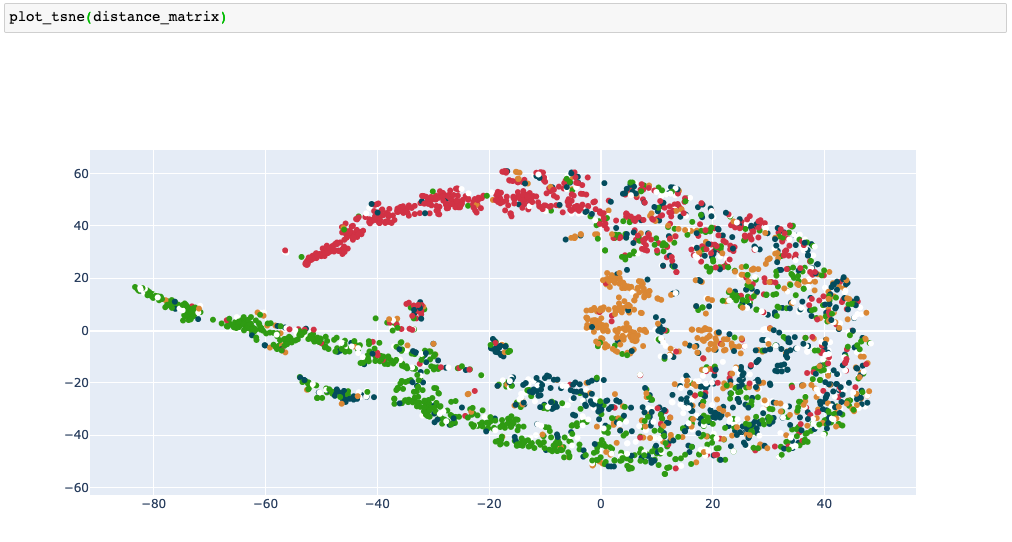
\includegraphics[width=\textwidth]{screenshots/our_word_movers_distance_tsne.png}
    \caption{Distance Matrix of the Word Mover's Distance with a self-trained model (plotted with t-SNE)}
    \label{fig:wmd-selftrained-1}
  \end{center}
\end{figure}
\FloatBarrier